\documentclass[11pt,a4paper]{report}

% ======================= FILL THESE IN BEFORE SUBMITTING =======================
\newcommand{\GitHubURL}{https://github.com/Anasnaveed69/23L-0764_A2_Ops}
\newcommand{\DagsHubURL}{https://dagshub.com/Anasnaveed69/23L-0764_A2_Ops}
\newcommand{\MLflowURL}{https://dagshub.com/Anasnaveed69/23L-0764_A2_Ops.mlflow}
\newcommand{\APIURL}{https://20-219-10-43.sslip.io}
\newcommand{\CommitHash}{9fbde8c}
\newcommand{\StudentName}{Anas Naveed Butt}
\newcommand{\RollNo}{23L-0764}
\newcommand{\Section}{7-D}
\newcommand{\Instructor}{Usman Anwer}
\newcommand{\SubmissionDate}{6 November 2026}
% ===============================================================================

\usepackage{amsmath}
\usepackage[T1]{fontenc}
\usepackage[utf8]{inputenc}
\IfFileExists{newtxtext.sty}{\usepackage{newtxtext,newtxmath}}{\usepackage{mathptmx}}  % Times New Roman
\usepackage[margin=2.3cm]{geometry}
\usepackage{graphicx,float,booktabs,array,tabularx,longtable}
\usepackage{xcolor,tcolorbox,enumitem,caption,subcaption}
\usepackage{titlesec}
\usepackage[hidelinks]{hyperref}
\usepackage[nameinlink,capitalise]{cleveref}
\usepackage{fancyhdr}
\usepackage{etoolbox}

\definecolor{vgblue}{HTML}{1F3A5F}
\definecolor{vgorange}{HTML}{E4572E}
\hypersetup{colorlinks=true,linkcolor=black,urlcolor=blue!60!black,citecolor=black}
\captionsetup{font=small,labelfont=bf}
\setlist{itemsep=2pt,topsep=4pt}
\setlength{\parskip}{4pt}
\sloppy\setlength{\emergencystretch}{3em}
\titleformat{\chapter}[hang]{\huge\bfseries}{\thechapter.}{12pt}{}
\titlespacing*{\chapter}{0pt}{-10pt}{18pt}
\titleformat{\section}{\Large\bfseries}{\thesection}{10pt}{}
\pagestyle{fancy}\fancyhf{}
\fancyhead[L]{\small VisionGuard (\RollNo)}\fancyhead[R]{\small\leftmark}
\fancyfoot[C]{\thepage}
\renewcommand{\headrulewidth}{0.4pt}

% ---------- helpers ----------
\graphicspath{{figures/}}
% Screenshot you take (figures/shots/<name>.png); grey placeholder until the file exists.
\newcommand{\shot}[3][0.92]{%
  \begin{figure}[H]\centering
  \IfFileExists{figures/shots/#2.png}{\includegraphics[width=#1\linewidth]{shots/#2.png}}{%
    \fcolorbox{gray}{gray!12}{\parbox[c][3.2cm][c]{#1\linewidth}{\centering\small\color{gray!70!black}
    \textbf{SCREENSHOT PENDING}\\[2pt]\texttt{figures/shots/\detokenize{#2}.png}\\[2pt]#3}}}
  \caption{#3}\label{fig:#2}\end{figure}}
% Figure produced by the scripts (figures/auto/<name>.png).
\newcommand{\autofig}[3][0.95]{%
  \begin{figure}[H]\centering
  \IfFileExists{figures/auto/#2.png}{\includegraphics[width=#1\linewidth]{auto/#2.png}}{%
    \fcolorbox{gray}{gray!12}{\parbox[c][3.2cm][c]{#1\linewidth}{\centering\small\color{gray!70!black}
    \textbf{GENERATED BY SCRIPT}\\[2pt]\texttt{figures/auto/\detokenize{#2}.png}}}}
  \caption{#3}\label{fig:#2}\end{figure}}
% Table produced by the scripts (generated/<name>.tex).
\newcommand{\gentable}[2]{%
  \begin{table}[H]\centering\small
  \IfFileExists{generated/#1.tex}{\input{generated/#1.tex}}{%
    \fcolorbox{gray}{gray!12}{\parbox{0.8\linewidth}{\centering\small\color{gray!70!black}
    \textbf{GENERATED BY SCRIPT}: \texttt{generated/\detokenize{#1}.tex}}}}
  \caption{#2}\label{tab:#1}\end{table}}
% Your own observation after looking at your real results.
\newtcolorbox{yourbox}{colback=yellow!12,colframe=orange!70!black,boxrule=0.6pt,arc=2pt,
  left=6pt,right=6pt,top=3pt,bottom=3pt,fontupper=\small}
\newcommand{\yours}[1]{\begin{yourbox}\textbf{Your observation:} #1\end{yourbox}}
\newcommand{\yoursize}{\textcolor{orange!70!black}{\textbf{[fill in]}}}
\newcommand{\cmd}[1]{\texttt{\detokenize{#1}}}
\newcommand{\file}[1]{\texttt{\detokenize{#1}}}
\newtcolorbox{wrongbox}[1][What went wrong]{colback=red!4,colframe=red!50!black,boxrule=0.5pt,arc=2pt,
  left=6pt,right=6pt,top=3pt,bottom=3pt,fontupper=\small,title=#1,
  fonttitle=\small\bfseries,coltitle=white,colbacktitle=red!50!black}

% numbers written by the scripts (defaults first, real values override)
% Fallback values shown until the scripts write report/generated/*_macros.tex
\newcommand{\vgPending}{\textbf{\textcolor{orange!70!black}{[run script]}}}
\newcommand{\vgNFiles}{\vgPending}\newcommand{\vgNReadable}{\vgPending}\newcommand{\vgNCorrupt}{\vgPending}
\newcommand{\vgNDup}{\vgPending}\newcommand{\vgNDupGroups}{\vgPending}\newcommand{\vgNConflicts}{\vgPending}
\newcommand{\vgNAI}{\vgPending}\newcommand{\vgNReal}{\vgPending}
\newcommand{\vgMedWAI}{\vgPending}\newcommand{\vgMedHAI}{\vgPending}\newcommand{\vgMedWReal}{\vgPending}
\newcommand{\vgMedHReal}{\vgPending}\newcommand{\vgMedKBAI}{\vgPending}\newcommand{\vgMedKBReal}{\vgPending}
\newcommand{\vgSquarePctAI}{\vgPending}\newcommand{\vgSquarePctReal}{\vgPending}
\newcommand{\vgNTrain}{\vgPending}\newcommand{\vgNVal}{\vgPending}\newcommand{\vgNTest}{\vgPending}
\newcommand{\vgNClean}{\vgPending}
\newcommand{\vgBaselineAccuracy}{\vgPending}\newcommand{\vgBaselinePrecision}{\vgPending}
\newcommand{\vgBaselineRecall}{\vgPending}\newcommand{\vgBaselineFOne}{\vgPending}
\newcommand{\vgBaselineRocauc}{\vgPending}\newcommand{\vgBaselineFalsepositiverate}{\vgPending}
\newcommand{\vgBaselineFalsenegativerate}{\vgPending}\newcommand{\vgBaselineBestEpoch}{\vgPending}
\newcommand{\vgBaselineThr}{\vgPending}\newcommand{\vgBaselineParams}{\vgPending}
\newcommand{\vgBaselineTrainable}{\vgPending}\newcommand{\vgBaselineValFpr}{\vgPending}
\newcommand{\vgBaselineAccHalf}{\vgPending}
\newcommand{\vgTransferAccuracy}{\vgPending}\newcommand{\vgTransferPrecision}{\vgPending}
\newcommand{\vgTransferRecall}{\vgPending}\newcommand{\vgTransferFOne}{\vgPending}
\newcommand{\vgTransferRocauc}{\vgPending}\newcommand{\vgTransferFalsepositiverate}{\vgPending}
\newcommand{\vgTransferFalsenegativerate}{\vgPending}\newcommand{\vgTransferBestEpoch}{\vgPending}
\newcommand{\vgTransferThr}{\vgPending}\newcommand{\vgTransferParams}{\vgPending}
\newcommand{\vgTransferTrainable}{\vgPending}\newcommand{\vgTransferValFpr}{\vgPending}
\newcommand{\vgTransferAccHalf}{\vgPending}
\newcommand{\vgBestRun}{\vgPending}\newcommand{\vgBestRunId}{\vgPending}\newcommand{\vgBestValAuc}{\vgPending}
\newcommand{\vgBestTestAuc}{\vgPending}\newcommand{\vgBestTestAcc}{\vgPending}\newcommand{\vgBestTestFone}{\vgPending}
\newcommand{\vgTunerTrials}{\vgPending}\newcommand{\vgTunerBestLr}{\vgPending}\newcommand{\vgTunerBestDrop}{\vgPending}
\newcommand{\vgTunerBestUnfrozen}{\vgPending}\newcommand{\vgTunerBestLoss}{\vgPending}
\newcommand{\vgTunerMostImportant}{\vgPending}

\makeatletter
\@for\vgf:={audit_macros,eda_macros,split_macros,baseline_macros,transfer_macros,best_macros,tuner_macros}\do{%
  \InputIfFileExists{generated/\vgf.tex}{}{}}
\makeatother

\begin{document}
\begin{titlepage}
\thispagestyle{empty}
\centering
\vspace*{1cm}
\IfFileExists{figures/fast_logo.png}{
\includegraphics[width=0.28\linewidth]{fast_logo.png}}{}\\[0.8cm]
{\LARGE National University of Computer and Emerging Sciences}\\[0.2cm]
{\Large Lahore Campus}\\[2.2cm]
{\Large MLOps}\\[0.3cm]
{\large Assignment 2}\\[1.6cm]
{\LARGE\bfseries VisionGuard: AI vs Real Image Classification}\\[2.4cm]
{\large Submitted by}\\[0.3cm]
{\Large \StudentName}\\[0.15cm]
{\large \RollNo \quad Section \Section}\\[1.4cm]
{\large Submitted to}\\[0.3cm]
{\Large \Instructor}\\[0.15cm]
\vfill
{\large Department of Computer Science}\\[0.15cm]
{\large \SubmissionDate}
\end{titlepage}

\pagenumbering{roman}
\chapter*{Project Information}
\addcontentsline{toc}{chapter}{Project Information}
\markboth{Project Information}{}

\section*{Links and graded version}
\renewcommand{\arraystretch}{1.35}
\begin{tabularx}{\linewidth}{>{\bfseries}l X}
\toprule
GitHub repository & \url{\GitHubURL} \\
DagsHub project (code, data, experiments, registry) & \url{\DagsHubURL} \\
MLflow tracking server & \url{\MLflowURL} \\
Live model API (cloud) & \url{\APIURL} \quad (\texttt{GET /health}, \texttt{POST /v1/predict}) \\
Web application & Flask on \texttt{http://localhost:5000} calling the API above (Task 8 design) \\
Commit hash of graded version & \texttt{\CommitHash} \\
\bottomrule
\end{tabularx}

\section*{System at a glance}
VisionGuard is a web service that estimates whether an uploaded image was produced by a generative
model or by a camera. The pipeline is: Kaggle dataset $\rightarrow$ audit and cleaning
$\rightarrow$ DVC-versioned data on DagsHub $\rightarrow$ \texttt{tf.data} pipeline $\rightarrow$
two Keras models (a CNN from scratch and a fine-tuned MobileNetV2) $\rightarrow$ every run tracked
in MLflow on DagsHub $\rightarrow$ the best model registered with alias \texttt{champion}
$\rightarrow$ a model API container on an Azure VM behind HTTPS $\rightarrow$ a Flask web app in
Docker Compose with a PostgreSQL audit trail, calling that API.

\begin{figure}[H]\centering\small
\setlength{\fboxsep}{6pt}
\begin{tabular}{c}
\fbox{\parbox{0.9\linewidth}{\centering
\textbf{Browser} $\;\rightarrow\;$ \textbf{Flask web app} (Docker, :5000) $\;\rightarrow\;$ \textbf{PostgreSQL} (internal network, named volume)\\[3pt]
\hspace*{3.2cm}$\downarrow$ HTTPS + \texttt{X-API-Key}\\[3pt]
\textbf{Azure VM}: Caddy (TLS) $\rightarrow$ gunicorn/Flask model API $\rightarrow$ \texttt{champion.keras} (TensorFlow-CPU)}}\\[6pt]
\fbox{\parbox{0.9\linewidth}{\centering
Kaggle $\rightarrow$ DVC (DagsHub storage) $\rightarrow$ \texttt{tf.data} $\rightarrow$ Keras $\rightarrow$
MLflow (DagsHub) $\rightarrow$ Registry \texttt{@champion} $\rightarrow$ \texttt{export\_champion.py} $\rightarrow$ image build}}
\end{tabular}
\caption{Serving path (top) and training path (bottom).}
\end{figure}

\section*{Disclosure of AI assistance and tutorials}
I used an AI assistant, Claude (Anthropic), extensively in this assignment:
\begin{itemize}
\item \textbf{Code}: Claude wrote most of the code in the repository (data scripts, training and
tracking code, Flask app, API, Dockerfiles, Compose files, CI workflow, Colab notebooks), which I
reviewed.
\item \textbf{Execution}: through the Claude desktop app, Claude operated my browser to run the
Colab notebooks, create the GitHub/DagsHub repositories and set up the Azure VM via Cloud Shell,
while I signed in to each service, created the access tokens and entered all secrets myself.
\item \textbf{Report}: Claude drafted the explanations in this report; I checked them against
my results and edited them. All numbers, tables and plots come from the actual runs (they are
written by the project scripts from MLflow and the evaluation code, not typed by hand).
\end{itemize}
Documentation consulted: TensorFlow/Keras guides (\texttt{tf.data}, transfer learning), MLflow,
DagsHub, DVC, Docker/Compose, GitHub Actions and Azure documentation.



\section*{How to read this report}
Each chapter is one task; each section is one sub-task ID from the assignment, and explains
\emph{what} I did, \emph{why}, \emph{how it works}, and \emph{what went wrong}. Every command is
explained where it is used. Tables marked as generated were written by the project scripts
(\file{report/generated/}) so the numbers cannot drift from the actual runs.

\tableofcontents
\clearpage
\pagenumbering{arabic}
\chapter{Data Understanding and Versioning}\label{ch:data}

\section{Environment}
\textbf{What and why.} I created an isolated virtual environment so the exact library versions
of this project cannot clash with other projects on my machine, and so anyone can rebuild the
same environment from \file{requirements.txt}. Every version is pinned (e.g.\ TensorFlow 2.20.0,
Keras 3.15.1, MLflow 2.22.5, Keras Tuner 1.4.7, DVC 3.67.1).

\textbf{How.} \cmd{py -3.11 -m venv .venv} creates a private copy of the interpreter and an empty
\cmd{site-packages}; activating it puts that interpreter first on \texttt{PATH}.
\cmd{pip install -r requirements.txt} installs the pinned set and \cmd{pip install -e .} installs
my own package \texttt{visionguard} (in \file{src/}) in editable mode so every script imports the
same code. \file{scripts/00_env_check.py} prints the user, host, Python, every library version,
whether the interpreter is inside a virtualenv, and what TensorFlow can see:
\cmd{tf.config.list_physical_devices("GPU")}. On my laptop TensorFlow sees only the CPU (native
Windows TensorFlow has no GPU support after 2.10), so the heavy training runs were executed on a
Colab T4 GPU with the same pinned tracking libraries (\cref{sec:2-0}).

\shot{s1_1_env}{Exact library versions, virtualenv check and GPU visibility (\file{scripts/00_env_check.py}).}

\textbf{Why MLflow 2.x and not 3.x?} MLflow 3 logs models through a new ``logged models'' REST
API. DagsHub's hosted tracking server implements the MLflow 2 API, so I pinned the client to the
latest 2.x release to keep \texttt{log\_model} and the Model Registry working against DagsHub.

\section{Dataset audit}
\textbf{What.} \file{scripts/01_audit.py} walks every file under \file{data/raw} and records, per
image: class (from the top-level folder name), file size, width, height, colour mode, format, a
SHA-256 hash of the bytes, whether the file can be fully decoded, and the error if not. The full
table is saved to \file{reports/audit/audit.csv}; summaries are written straight into this report.

\textbf{How each check works.}
\begin{itemize}
\item \emph{Readability}: \texttt{PIL.Image.verify()} catches broken headers and \texttt{load()}
forces a full pixel decode, which catches truncated files that open fine but fail later.
I deliberately use the \emph{same} decode function as training and serving
(\file{src/visionguard/imaging.py}), so ``readable'' in the audit means ``usable by the model''.
\item \emph{Duplicates}: two files are exact duplicates when their SHA-256 hashes are equal (same
bytes). I keep the first copy only. Duplicates matter because a copy in the training set and
another in the test set leaks the answer and inflates test accuracy.
\item \emph{Label conflicts}: a hash that appears under \emph{both} classes is label noise; all
copies are dropped.
\item Images smaller than 32 pixels on a side are flagged as unusable.
\end{itemize}

\gentable{audit_counts}{Files per class: total, readable, corrupt (cannot be decoded), exact duplicates and too-small images.}
\gentable{audit_stats}{Minimum, median and maximum of width, height and file size per class (readable files only).}
\gentable{audit_formats}{Image formats and colour modes per class.}

The dataset has \vgNFiles{} files: \vgNAI{} AI-generated and \vgNReal{} real. \vgNCorrupt{}
files could not be decoded and \vgNDup{} are exact duplicates (\vgNDupGroups{} duplicate groups,
\vgNConflicts{} hashes appearing in both classes). After cleaning, \vgNClean{} images remain and
are split 70/15/15 with stratification (same AI/real ratio in every split), using a fixed seed:

\gentable{splits}{Stratified train / validation / test split after removing corrupt files, duplicates and label conflicts.}
\gentable{audit_corrupt}{Files that could not be decoded (first 15) and the decoder's error.}

\shot{s1_2_audit}{Terminal output of the audit script.}

\begin{wrongbox}[Problem I had to design around]
The obvious decoder, \texttt{tf.io.decode\_image}, cannot read WEBP files, CMYK JPEGs or
palette PNGs with transparency, all of which occur in scraped data. Using it would have marked good
images as ``corrupt'' and thrown them away, so the audit, training and serving all use one Pillow
function that converts every image to RGB (compositing transparency onto white so transparent
pixels do not turn black).
\end{wrongbox}

\section{Visual EDA}
\autofig{eda_samples}{Random samples per class (top two rows AI-generated, bottom two rows real), with original size and format.}
\textbf{Interpretation.} The AI-generated images are mostly polished, centred compositions with
smooth gradients, glossy lighting and an ``illustration'' look, while the real images include
everyday clutter, uneven exposure and natural noise. Both classes contain people, animals and
landscapes, so the model cannot solve the task by topic alone; it has to use style and texture.

\autofig{eda_histograms}{Width, height, file size (log scale) and aspect ratio per class.}
\textbf{Interpretation.} The median AI image is \vgMedWAI{}$\times$\vgMedHAI{} pixels and
\vgMedKBAI{}\,KB, versus \vgMedWReal{}$\times$\vgMedHReal{} pixels and \vgMedKBReal{}\,KB for real
images. \vgSquarePctAI{}\% of AI images are exactly square against \vgSquarePctReal{}\% of real
ones, because generators output fixed square resolutions. These differences are a
\emph{shortcut risk}: a network could learn ``square and small file $\Rightarrow$ AI'' instead of
learning generation artefacts. Resizing every image to the same square input removes the size
signal from the pixels, but compression strength still differs; I return to this in the error
analysis (\cref{sec:2-6}).

\yours{After running \file{02_eda.py} on the real data, check that the two paragraphs above still
match your figures (e.g.\ which class is larger, how strong the square-image peak is) and adjust a
sentence if not.}

\section{Data version control with DVC}
\subsection*{Toy exercise}
\textbf{What and why.} In an empty folder I created a 3-row \file{scores.csv}, versioned it with
DVC, changed it, travelled back to the old version, and round-tripped it through remote storage
on DagsHub (repository \texttt{23L-0764\_A2\_Ops-dvc-toy}). Commands, in order
(\file{labs/dvc_toy.sh}):
\begin{enumerate}
\item \cmd{git init}, \cmd{dvc init}: Git tracks code and small text; DVC adds \file{.dvc/}
(config + local cache) on top of Git.
\item \cmd{dvc add scores.csv}: moves the content into the content-addressed cache
\file{.dvc/cache/<md5>} and writes the pointer \file{scores.csv.dvc}; it also adds
\file{scores.csv} to \file{.gitignore} so Git never stores the data itself. I commit the pointer.
\item Append two rows, \cmd{dvc add} again, commit: the pointer now holds a different md5.
\item \cmd{git checkout HEAD~1 -- scores.csv.dvc} restores the old pointer and
\cmd{dvc checkout} replaces the workspace file with the cached content for that md5: the 3-row
version is back. Git chooses \emph{which} version; DVC supplies the \emph{bytes}.
\item \cmd{dvc remote add -d origin s3://dvc} plus \cmd{endpointurl} points DVC at DagsHub's
S3-compatible storage; the token is set with \cmd{--local}, which writes it to
\file{.dvc/config.local} (git-ignored) instead of the committed \file{.dvc/config}.
\item \cmd{dvc push --all-commits} uploads the data for every committed version. I then deleted
\file{scores.csv} \emph{and} the local cache, and \cmd{dvc pull} downloaded it again.
\end{enumerate}

\shot{s1_4_toy_pointer}{The pointer file and the two commits (v1, v2).}
\shot{s1_4_toy_checkout}{Returning to the older version with \cmd{git checkout} + \cmd{dvc checkout}.}
\shot{s1_4_toy_pushpull}{Push to DagsHub, delete local data and cache, pull it back.}
\shot{s1_4_toy_dagshub}{The toy repository on DagsHub with the DVC-tracked file.}

\subsection*{What the pointer file holds, and why data does not belong in Git}
The \file{.dvc} file is a few lines of YAML: the \texttt{md5} of the content (for a directory, the
md5 of a manifest listing every file and its hash), the total \texttt{size}, the number of files
and the \texttt{path}. It is a fingerprint, not data. Git is built for small text that changes
line by line: every version of every file is stored forever in \file{.git}, so committing
hundreds of megabytes of images makes every clone download all of it, binary diffs are
meaningless, and GitHub rejects files over 100\,MB. With DVC, Git history stays tiny, and the
data version is the md5 in the pointer, which I also log to MLflow as the tag
\texttt{dvc\_data\_version}, so every experiment says exactly which data it used.

\subsection*{Applying it to VisionGuard}
\cmd{dvc add data/raw} tracks the whole dataset directory as one unit (\file{data/raw.dvc}),
with DagsHub storage of the \texttt{23L-0764\_A2\_Ops} repository as the default remote. The
split lists (\file{data/splits/*.csv}, a few KB) are committed to Git directly, because they
are small text and must change together with the code that produced them.

\shot{s1_4_dataset_dvc}{\cmd{dvc add data/raw}, commit of the pointer, and \cmd{dvc push} of the dataset.}
\shot{s1_4_dagshub_data}{DagsHub repository page showing \file{data/raw} tracked by DVC.}

\begin{wrongbox}[Problems to watch for]
A plain \cmd{dvc push} uploads only the data of the \emph{current} commit, so after deleting the
cache an older version could not be restored from the remote; \cmd{dvc push --all-commits}
uploads every version referenced in Git history. The second trap is credentials:
\cmd{dvc remote modify} without \cmd{--local} writes the token into \file{.dvc/config}, which is
committed, so the token would be published.
\end{wrongbox}

\chapter{Model Development with TensorFlow/Keras}\label{ch:model}

\section*{Where training ran}\label{sec:2-0}
All model code lives in \file{src/visionguard/} and is driven by \file{scripts/train.py}; every
setting comes from \file{params.yaml} and can be overridden per run
(\cmd{--set train.lr_head=0.0001}). Data preparation ran on my laptop; the training runs ran on a
Google Colab T4 GPU (\file{notebooks/train_colab.ipynb}), which clones the same commit from GitHub
and pulls the same data version with \cmd{dvc pull}, so a run is fully identified by the
\texttt{git\_commit} and \texttt{dvc\_data\_version} tags it logs.

\section{Input pipeline}
\textbf{Stages} (\file{src/visionguard/data.py}, \texttt{make\_dataset}):
\begin{enumerate}
\item \textbf{List}: \texttt{from\_tensor\_slices((paths, labels))} from the split CSV. Reading
the split lists, not the folders, guarantees the same images land in the same split every time.
\item \textbf{Decode + resize} (parallel): \texttt{tf.numpy\_function} calls the shared Pillow
function \texttt{decode\_and\_resize} with \texttt{num\_parallel\_calls=AUTOTUNE}. The output is a
$224\times224\times3$ tensor of raw 0--255 values.
\item \textbf{Cache}: the decoded images are cached in RAM after the first epoch as
\texttt{uint8} (4$\times$ smaller than \texttt{float32}), so JPEG decoding happens once.
\item \textbf{Shuffle} (training only): buffer = whole training set, fixed seed, reshuffled every epoch.
\item \textbf{Batch} (32) and \textbf{augment} (training only, applied to whole batches):
horizontal flip, rotation $\pm$5\%, zoom $\pm$10\%, translation $\pm$5\%, contrast $\pm$10\%.
\item \textbf{Prefetch}: the CPU prepares the next batch while the GPU trains on the current one.
\end{enumerate}
Validation and test data go through the same stages without shuffle and augmentation, so they
are evaluated exactly as they are.

\textbf{Image size.} 224\,px is the resolution MobileNetV2 was pre-trained on, so its filters
see objects at the scale they learned; it also keeps the batch cheap. One experiment uses
160\,px to measure the effect (\cref{sec:3-5}).

\textbf{Aspect ratio.} The default resize \emph{squashes} every image to a square, so a
$1000\times500$ photo is compressed horizontally by 2$\times$ and its aspect ratio is lost. The
alternative (\texttt{resize\_mode: pad}) keeps the ratio and pads with black bars, but then the
amount of padding itself tells the model the original shape, which is one of the shortcuts found
in the EDA. I kept squashing for both classes so the shape signal is neutral.

\textbf{Augmentation choices.} The augmentations change geometry and global contrast but keep
fine texture. I deliberately avoided blur, noise and JPEG re-compression: those destroy the
high-frequency artefacts that distinguish generated images, and could turn an AI image into
something that statistically looks like a camera image while keeping the ``AI'' label.

\autofig{batch_plain}{A training batch after decode + resize, before augmentation.}
\autofig{batch_augmented}{The same batch after the training-time augmentation.}

\section{Baseline CNN from scratch}
\textbf{Architecture} (\file{models.py}, \texttt{build\_baseline}). Every layer has a job:
\begin{itemize}
\item \textbf{Rescaling(1/255)}: maps pixels to $[0,1]$ inside the model, so serving code only
sends raw pixels and cannot forget the scaling.
\item \textbf{4 blocks of Conv2D(3$\times$3) $\rightarrow$ BatchNorm $\rightarrow$ ReLU
$\rightarrow$ MaxPool(2)} with 32, 64, 128, 256 filters: convolutions learn local patterns
(edges, then textures, then parts); doubling filters while halving resolution keeps compute
balanced; BatchNorm normalises activations so training is stable with a higher learning rate
(the conv has \texttt{use\_bias=False} because BN's shift replaces the bias); ReLU adds
non-linearity; pooling gives translation tolerance and grows the receptive field.
\item \textbf{GlobalAveragePooling}: averages each feature map to one number, turning
$14\times14\times256$ into 256 values. Far fewer parameters than \texttt{Flatten} + Dense, which
matters with only a few hundred training images.
\item \textbf{Dropout(0.4)}, \textbf{Dense(64, ReLU)}, \textbf{Dropout(0.2)}: a small
classifier head; dropout randomly zeroes units during training to reduce over-fitting.
\item \textbf{Dense(1, sigmoid)}: one output $p = P(\text{AI}\mid\text{image})$.
\end{itemize}

\textbf{Loss, optimiser, metrics.} Binary cross-entropy is the negative log-likelihood of a
Bernoulli output, the natural loss for one sigmoid unit, and it rewards calibrated probabilities
(which I need, because the threshold is chosen later). Adam with learning rate $10^{-3}$ adapts
per-parameter step sizes and works well without tuning on small CNNs. Metrics: accuracy (easy to
read), ROC-AUC (threshold-free ranking quality), precision and recall of the AI class (the two
error types of \cref{sec:2-5}). Inverse-frequency class weights stop the model from ignoring the
smaller class.

\gentable{baseline_layers}{Baseline CNN: output shape and parameter count per layer (\vgBaselineParams{} parameters).}
\shot{s2_2_summary}{\texttt{model.summary()} of the baseline CNN.}

\section{Transfer learning (MobileNetV2)}
\textbf{Why MobileNetV2.} Its depthwise-separable convolutions give good ImageNet features with
only about 2.3\,M backbone parameters (14\,MB on disk), so it fine-tunes quickly on a small
dataset and runs fast on the CPU-only server. It is loaded with
\cmd{keras.applications.MobileNetV2(include_top=False, weights="imagenet")}: no 1000-class
classifier, just the convolutional feature extractor ending in a $7\times7\times1280$ map.

\textbf{Preprocessing.} MobileNetV2 was trained on pixels scaled to $[-1,1]$
(\texttt{mobilenet\_v2.preprocess\_input} computes $x/127.5-1$). Feeding $[0,1]$ or $[0,255]$
would shift every activation away from what the pre-trained filters expect and destroy the value
of the weights. I put this scaling inside the model as \texttt{Rescaling(1/127.5, offset=-1)},
so the saved model always applies it, in training and in serving. (EfficientNetB0, used in one
experiment, contains its own normalisation and expects raw 0--255, so it gets an identity layer.)

\textbf{Head.} GlobalAveragePooling $\rightarrow$ Dropout(0.3) $\rightarrow$ Dense(1, sigmoid).

\textbf{Stage 1 (frozen backbone).} \texttt{base.trainable = False}; only the head
(1\,281 weights) learns, at learning rate $10^{-3}$. Random head weights produce large
gradients; if the backbone were trainable, those gradients would wreck the pre-trained filters.

\textbf{Stage 2 (last block unfrozen).} Only the layers of MobileNetV2's last inverted-residual
block (\texttt{block\_16}) and the final \texttt{Conv\_1} are made trainable:
\IfFileExists{generated/transfer_unfrozen.tex}{\texttt{block\_16\_expand}, \texttt{block\_16\_expand\_relu}, \texttt{block\_16\_depthwise}, \texttt{block\_16\_depthwise\_relu}, \texttt{block\_16\_project}, \texttt{Conv\_1}, \texttt{out\_relu}}{\vgPending}.
The model is recompiled (required for the change to take effect) with a learning rate 100$\times$
smaller ($10^{-5}$), so the high-level features adapt to generator artefacts without forgetting
ImageNet. BatchNorm layers stay frozen and the backbone is called with \texttt{training=False}:
otherwise BN would replace ImageNet statistics with statistics from batches of 32 images.

\gentable{transfer_trainable}{Trainable weights in each stage.}
\autofig{transfer_stage1_curves}{Stage 1 (frozen backbone): loss and accuracy.}
\autofig{transfer_stage2_curves}{Stage 2 (last block unfrozen, learning rate $10^{-5}$): loss and accuracy.}
\gentable{transfer_layers}{Transfer model, top-level layers (\vgTransferParams{} parameters in total, \vgTransferTrainable{} trainable in stage 2).}

\begin{wrongbox}
In Keras 3, renaming the backbone with \texttt{base.\_name = "backbone"} silently had no effect,
so \texttt{model.get\_layer("backbone")} failed when unfreezing. Passing \texttt{name="backbone"}
to the constructor fixed it.
\end{wrongbox}

\section{Training discipline}
\begin{itemize}
\item \textbf{Seeds}: \cmd{keras.utils.set_random_seed(42)} seeds Python, NumPy and TensorFlow
together; \texttt{PYTHONHASHSEED} is fixed; the split, the shuffle and every augmentation layer
get explicit seeds. (GPU kernels are not bit-exact, so reruns on a GPU can differ in the third
decimal; the seed is logged as a tag on every run.)
\item \textbf{EarlyStopping} on \texttt{val\_loss}, patience 4, \texttt{restore\_best\_weights=True}.
\item \textbf{ModelCheckpoint} on \texttt{val\_loss} with \texttt{save\_best\_only}. One checkpoint
object is shared by both transfer stages, so it keeps the best epoch \emph{across} stages; after
training I reload that file, so the evaluated model is the best one, not the last one.
\item \textbf{ReduceLROnPlateau}: multiplies the learning rate by 0.3 after 2 epochs without
improvement in \texttt{val\_loss}.
\end{itemize}
Best epochs (lowest validation loss): baseline CNN \textbf{epoch \vgBaselineBestEpoch}, transfer
model \textbf{epoch \vgTransferBestEpoch} (counted across both stages).

\autofig{baseline_curves}{Baseline CNN: loss and accuracy, best epoch marked in red.}
\autofig{transfer_curves}{Transfer model, both stages: best epoch in red, start of fine-tuning dotted.}

\yours{Describe what the curves show, e.g.\ whether validation loss flattened before training
loss (over-fitting) and whether stage 2 lowered validation loss further.}

\section{Evaluation}\label{sec:2-5}
\textbf{Which error is worse?} A \emph{false positive} (a real photo called AI-generated) is
worse for this product. VisionGuard would be used to judge whether someone's photo is genuine; a
false accusation harms a real person (a journalist, a seller, a student) and destroys trust in the
tool. A false negative (an AI image passing as real) is bad but is the status quo without the
tool. So I want high \emph{precision} on the AI class, i.e.\ a low false-positive rate.

\textbf{Threshold.} The test set is used once, at the end. The threshold is chosen on the
\emph{validation} predictions: I scan $t\in[0.05,0.95]$ and pick the value that maximises
$F_{\beta}$ with $\beta=0.5$, which weights precision twice as much as recall and therefore
encodes the choice above. Chosen thresholds: baseline \vgBaselineThr, transfer \vgTransferThr.
The threshold is saved with the model (\file{model_meta.json}) and used by the server.

\gentable{model_metrics}{Test-set metrics at the validation-chosen threshold (FPR = real photos called AI).}

\begin{figure}[H]\centering
\begin{subfigure}{0.45\linewidth}\centering
\IfFileExists{figures/auto/baseline_confusion_matrix.png}{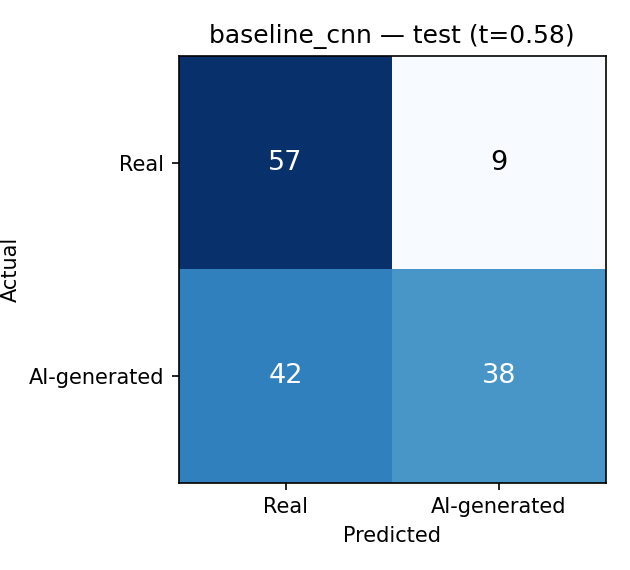
\includegraphics[width=\linewidth]{auto/baseline_confusion_matrix.png}}{\fbox{\parbox[c][3cm][c]{0.9\linewidth}{\centering generated}}}
\caption{Baseline CNN}\end{subfigure}\hfill
\begin{subfigure}{0.45\linewidth}\centering
\IfFileExists{figures/auto/transfer_confusion_matrix.png}{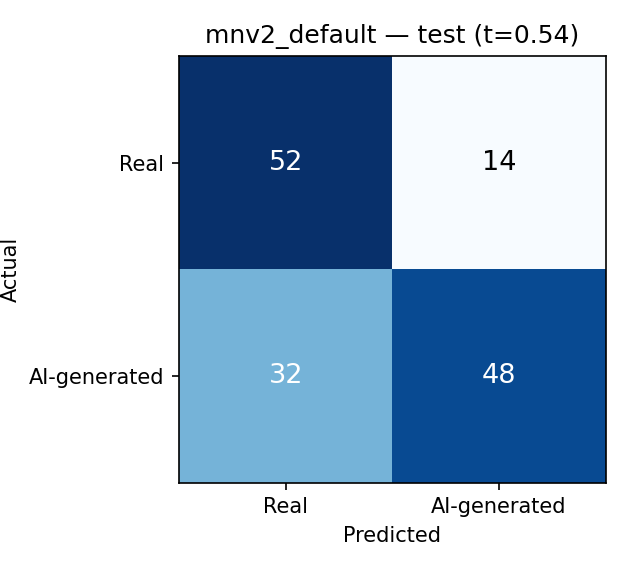
\includegraphics[width=\linewidth]{auto/transfer_confusion_matrix.png}}{\fbox{\parbox[c][3cm][c]{0.9\linewidth}{\centering generated}}}
\caption{MobileNetV2 transfer}\end{subfigure}
\caption{Test confusion matrices.}\label{fig:cms}\end{figure}

\begin{figure}[H]\centering
\begin{subfigure}{0.45\linewidth}\centering
\IfFileExists{figures/auto/baseline_roc_curve.png}{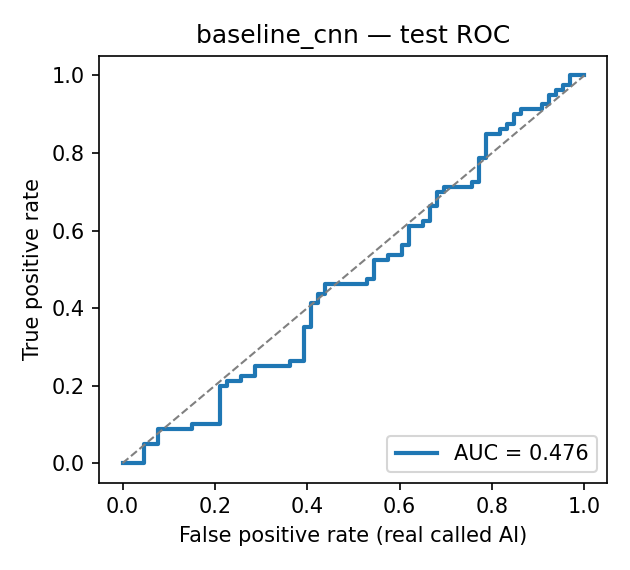
\includegraphics[width=\linewidth]{auto/baseline_roc_curve.png}}{\fbox{\parbox[c][3cm][c]{0.9\linewidth}{\centering generated}}}
\caption{Baseline CNN}\end{subfigure}\hfill
\begin{subfigure}{0.45\linewidth}\centering
\IfFileExists{figures/auto/transfer_roc_curve.png}{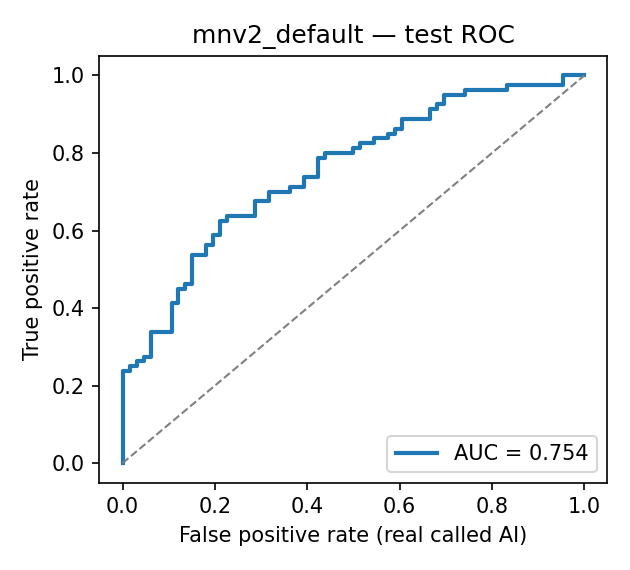
\includegraphics[width=\linewidth]{auto/transfer_roc_curve.png}}{\fbox{\parbox[c][3cm][c]{0.9\linewidth}{\centering generated}}}
\caption{MobileNetV2 transfer}\end{subfigure}
\caption{Test ROC curves.}\label{fig:rocs}\end{figure}

The transfer model reaches test accuracy \vgTransferAccuracy{}, F1 \vgTransferFOne{} and ROC-AUC
\vgTransferRocauc{}, with a false-positive rate of \vgTransferFalsepositiverate{}; the
baseline reaches \vgBaselineAccuracy{}, \vgBaselineFOne{} and \vgBaselineRocauc{} (FPR
\vgBaselineFalsepositiverate{}).

\yours{One or two sentences: which model is better and by how much; is the gap mainly in AUC (ranking)
or at the threshold? Pre-trained features usually win clearly on a dataset this small.}

\section{Error analysis}\label{sec:2-6}
\file{scripts/error_analysis.py} takes the champion's test predictions, keeps the ten most
\emph{confident} mistakes (the most informative ones), and measures simple properties of each:
size, sharpness (variance of an edge filter), colour saturation, grey-scale, aspect ratio and
format. These give each error a testable hypothesis instead of a guess.

\autofig{errors_grid}{The ten most confident test errors (true label, prediction, $p(\text{AI})$, size).}
\gentable{errors}{Measured cues and hypothesis per error.}

\yours{Look at each of the 10 images and confirm or correct its hypothesis (e.g.\ watermark,
painting style, text in the image, heavy JPEG artefacts, a real photo of a CGI scene). Note any
pattern, e.g.\ ``most false positives are smooth, studio-lit portraits''.}

\section{Tool lab: Keras Tuner}
\subsection*{Toy part}
\file{labs/tuner_toy.py} tunes a one-hidden-layer network on Fashion-MNIST with
\textbf{Hyperband}: number of units $\in\{32,\dots,512\}$ and learning rate
$\in\{10^{-2},10^{-3},10^{-4}\}$. Hyperband trains many configurations for a few epochs,
keeps the best third, trains those longer, and repeats, so most of the budget goes to promising
settings. \cmd{tuner.get_best_hyperparameters()} returns the winner.
\gentable{tuner_toy}{Toy tuner: best trials on Fashion-MNIST (validation accuracy).}
\shot{s2_7_toy_tuner}{Toy tuner results summary.}

\subsection*{Applied to VisionGuard}
\file{scripts/tune.py} defines a \texttt{HyperModel} whose \texttt{fit()} reproduces the two-stage
training inside each trial and searches the head learning rate (log-uniform
$10^{-4}$--$3\cdot10^{-3}$), dropout (0.1--0.5) and how many backbone layers to unfreeze
$\in\{0, 11\ (\text{last block}), 30, 60\}$ with \textbf{RandomSearch}, \vgTunerTrials{} trials,
objective validation loss. Every trial is also logged to MLflow as a nested run.

\gentable{tuner_trials}{VisionGuard tuner trials, best first.}
\autofig[0.95]{tuner_effects}{Validation loss of each trial against each hyper-parameter.}
\gentable{tuner_effects}{Effect size: spread of mean validation loss across the levels of each hyper-parameter.}
\shot{s2_7_tuner}{Tuner search output for VisionGuard.}

Best trial: learning rate \vgTunerBestLr, dropout \vgTunerBestDrop, \vgTunerBestUnfrozen{}
unfrozen layers (validation loss \vgTunerBestLoss). The hyper-parameter with the largest effect
was \textbf{\vgTunerMostImportant}.

\yours{One sentence on why that hyper-parameter mattered most (e.g.\ the learning rate controls
whether the new head converges in a few epochs; unfreezing many layers on ~600 images over-fits).}

\textbf{Why the best validation score can over-fit the validation set.} The tuner looks at the
validation loss of every trial and keeps the minimum. With many trials, some configurations score
well partly by luck on this particular, small validation set (a ``winner's curse''): selection
itself fits noise in the validation data, so the best score is an optimistic estimate. That is
why the final numbers come from the untouched test set, used once, and why a clearly simpler
setting within noise of the best is a reasonable choice.

\section*{Bonus: Grad-CAM}
\autofig{gradcam}{Grad-CAM heat maps: top row correct predictions, bottom row errors. Red = regions that pushed $p(\text{AI})$ up.}
Grad-CAM takes the gradient of the output with respect to the last convolutional feature map,
averages it per channel to get channel weights, and shows the weighted sum of the feature maps as
a heat map.

\yours{Comment on what the model looks at, e.g.\ skin/hair texture and backgrounds for AI
portraits (where generators leave smooth, repetitive texture), versus edges of objects or
watermark areas in the errors.}

\chapter{Experiment Tracking with MLflow and DagsHub}\label{ch:tracking}

\section{Tool lab: MLflow locally}
\file{labs/mlflow_toy.py} trains a network with one hidden layer on 10\,000 Fashion-MNIST images.
It logs the parameters (\texttt{lr}, \texttt{epochs}, \texttt{units}, \texttt{optimizer}), the
per-epoch metrics through a small Keras callback (\texttt{mlflow.log\_metrics(..., step=epoch)}),
a loss plot (\texttt{mlflow.log\_figure}) and the model (\texttt{mlflow.tensorflow.log\_model}). I
ran it twice, with \texttt{lr=0.001} and \texttt{lr=0.01}, against a local store (\cmd{--local}
writes to \file{./mlruns_toy}), and then opened \cmd{mlflow ui --backend-store-uri ./mlruns_toy}.
The comparison view overlays the two \texttt{val\_accuracy} curves and highlights the parameter
that differs. These two runs ran on CPU in a separate Linux workspace (TensorFlow 2.20, MLflow
2.22.5) with the UI on \texttt{127.0.0.1}.

After 5 epochs the higher learning rate fits the training data faster (training accuracy 0.862
against 0.849, loss 0.373 against 0.437) but does no better on validation (0.842 against 0.846),
so I would keep \texttt{lr=0.001}.

\shot{s3_1_mlflow_runs}{Local MLflow UI: the toy experiment with both runs.}
\shot{s3_1_mlflow_compare}{Comparison of the two learning rates.}

In my own words, the MLflow terms are:
\begin{description}[leftmargin=2.2cm,style=nextline]
\item[Experiment] a named group of runs working on the same problem, so they can be compared side
by side. Here I have \texttt{VisionGuard} and \texttt{toy-fashion-mnist}.
\item[Run] one execution of the training code. It has a unique id, a start and end time and a
status, and everything logged while it runs belongs to it.
\item[Parameter] an input setting that is fixed for the run and written once, such as the learning
rate. Parameters cannot be changed: logging a different value for the same key raises an error.
\item[Metric] a numeric result that can be logged many times with a step, for example
\texttt{val\_loss} after every epoch. This is how MLflow draws the curves.
\item[Artifact] any output file stored with the run, such as plots, CSVs, the requirements list or
the model itself.
\item[Tag] free-form key/value information that describes the run without configuring it, such as
the git commit, the data version or who ran it. Tags can be edited later and are useful for
searching.
\end{description}

\section{DagsHub setup}
I created the DagsHub project \texttt{23L-0764\_A2\_Ops} with ``Connect a repository'', so it
mirrors my GitHub repository and adds DVC storage and a hosted MLflow server. The tracking address
is \url{\MLflowURL}, but it does not appear anywhere in the code. \file{tracking.py} calls
\texttt{load\_dotenv()} and reads \texttt{MLFLOW\_TRACKING\_URI}, and MLflow reads
\texttt{MLFLOW\_TRACKING\_USERNAME} and \texttt{MLFLOW\_TRACKING\_PASSWORD} (the DagsHub token) from
the environment. These values are in \file{.env}, which is listed in \file{.gitignore} and
\file{.dockerignore}, and \file{.env.example} shows the variable names with dummy values. If
\texttt{MLFLOW\_TRACKING\_URI} is not set, the code falls back to a local \file{mlruns/} folder, so
it still works offline.

\shot{s3_2_dagshub_project}{The DagsHub project connected to GitHub.}
\shot{s3_2_dagshub_toy_run}{The toy run logged to DagsHub's MLflow server.}
\shot{s3_2_gitignore}{\file{.env} is git-ignored: \cmd{git check-ignore -v .env} names the rule and \cmd{git status} does not list it.}

\section{Instrumenting VisionGuard training}
Each run of \file{scripts/train.py} logs:
\begin{itemize}
\item every value from \file{params.yaml} that was actually used, flattened into names like
\texttt{train.lr\_head}, plus the split sizes and class weights, as parameters;
\item loss, accuracy, AUC, precision and recall for training and validation after every epoch, and
the learning rate, so ReduceLROnPlateau shows up in the curves;
\item final metrics: \texttt{best\_epoch}, the chosen \texttt{val\_threshold}, all validation and
test metrics at that threshold (\texttt{test\_accuracy}, \texttt{test\_f1},
\texttt{test\_roc\_auc}, \texttt{test\_false\_positive\_rate}, the confusion-matrix cells), and
test accuracy and F1 at the plain 0.5 threshold for comparison;
\item tags: \texttt{git\_commit}, \texttt{git\_dirty}, \texttt{dvc\_data\_version} (the md5 from
\file{data/raw.dvc}), \texttt{seed}, the Python, TensorFlow and Keras versions, the platform, model
type, backbone and tracking mode.
\end{itemize}

With manual tracking (\cmd{--tracking manual}, for example the run \texttt{mnv2\_default}) my
callback \texttt{MLflowEpochLogger} passes Keras' \texttt{logs} to \texttt{mlflow.log\_metrics}
at the end of every epoch with a global step, so the two training stages form one continuous curve.
With autologging (\cmd{--tracking autolog}, run \texttt{mnv2\_autolog}),
\texttt{mlflow.tensorflow.autolog()} patches \texttt{model.fit()} and records things by itself.

\begin{table}[H]\centering\small
\begin{tabularx}{\linewidth}{l X X}
\toprule
 & Manual callback & Autologging \\
\midrule
Captures & exactly what I choose: per-epoch metrics and LR, my parameters and tags & every \texttt{fit()} argument (epochs, batch size, class weight\ldots), all optimizer settings (\texttt{opt\_*}), per-epoch metrics, model summary and EarlyStopping info, with no extra code \\
Misses & anything I forget to log & test metrics, the chosen threshold, git/DVC tags, the confusion matrix and the splits, because it only sees \texttt{fit()} \\
Two-stage training & one continuous run & the second \texttt{fit()} tries to log \texttt{epochs} again with a new value, which is not allowed, so I put stage 2 in a nested child run \\
Clutter & short & many parameters that have nothing to do with the experiment \\
\bottomrule
\end{tabularx}
\caption{Manual logging versus autologging.}\end{table}

In practice I would use both together: autolog for what happens inside training, and explicit
logging for provenance and evaluation. Both kinds of run here came from the same configuration.

\shot{s3_3_manual_run}{Manual run: parameters, metric curves and provenance tags.}
\shot{s3_3_autolog_run}{Autologged run: the automatically captured \texttt{fit()} and optimizer parameters.}

I hit two errors while setting this up. MLflow rejected my first metric name,
\texttt{test@0.5\_accuracy}, because metric names may only contain letters, digits, \texttt{\_ - .
/ :} and spaces, so I renamed it to \texttt{test\_t0.5\_accuracy}. Then the first autolog run had
no epoch metrics at all. Autolog tried to log \texttt{class\_weight}, which I had already logged
under the same key in a different string format, and because parameters cannot change, the autolog
hook gave up. I renamed my parameter to \texttt{class\_weights} and moved the second \texttt{fit()}
into a nested run.

\section{Artifacts}
Each run stores \file{plots/} (training curves, confusion matrix, ROC curve), \file{splits/} (the
exact train, validation and test CSVs), \file{environment/} (\file{requirements-freeze.txt} from
\cmd{pip freeze}, and \file{params.yaml}), \file{evaluation/test_predictions.csv},
\file{model_info/} (model summary and the trainable layers per stage), \file{keras_model/} (the
\file{model.keras} file and \file{model_meta.json} with image size, resize mode and threshold) and
\file{model/}, the MLflow TensorFlow-flavour model with an input/output signature that the registry
uses.

\shot{s3_4_artifacts}{Artifacts tab of the champion run.}

\section{Experiment comparison}\label{sec:3-5}
\file{scripts/run_experiments.py} launches the reference run and a set of variants, each changing
one thing compared with the reference, so any difference can be put down to that change.
\file{scripts/compare_runs.py} pulls all finished runs from MLflow and builds the table and the
chart.

\gentable{runs}{All VisionGuard runs (sorted by validation ROC-AUC).}
\autofig{runs_comparison}{Validation ROC-AUC and test F1 per run.}
\shot{s3_5_compare}{MLflow/DagsHub run comparison view.}

I pick the model by validation ROC-AUC, which does not depend on a threshold and measures how well
the model ranks AI images above real ones. Ties are broken by the validation false-positive rate,
since false accusations are the expensive error. The test metrics are in the table but play no part
in the choice; otherwise the test set would turn into a second validation set. The chosen run is
\texttt{\vgBestRun}, with validation AUC \vgBestValAuc, test AUC \vgBestTestAuc, test accuracy
\vgBestTestAcc{} and test F1 \vgBestTestFone.

Starting the transfer stage from the tuner's settings helped the most (validation AUC from 0.830 to
0.881, test F1 from 0.676 to 0.731). Turning augmentation off also improved the validation AUC, to
0.859. On a dataset this small the random flips, rotations and zoom mostly slowed learning down,
and zoom and rotation also change the fine generator textures the model depends on. The 160\,px
input did worst on the selection metric (validation AUC 0.764, validation FPR 0.29), since
shrinking the image wipes out fine texture. It had a higher test accuracy, but on 146 images that
is noise, and the selection rule ignores it on purpose. EfficientNetB0 had the best test AUC
(0.852) but a lower validation AUC, so I did not choose it. The autolog run matches the manual
reference (validation AUC 0.830 for both; test AUC 0.764 against 0.754, because GPU training is
not bit-exact).

My first version of the comparison ranked runs by \texttt{val\_auc}. That is the Keras AUC from the
last epoch the callback logged, which is not the best checkpoint that actually gets evaluated, and
autologged runs did not have it with the same meaning. I switched to \texttt{val\_roc\_auc}, which
my evaluation code computes on the reloaded best model for every run.

\section{Model registry}
\file{scripts/register_model.py} makes sure the registered model \texttt{VisionGuard-23L-0764} has
at least two versions. The reference transfer run and the baseline CNN are registered during
training with \cmd{--register}, and the selected run is registered if it is not there yet. The
script gives the best version the alias \texttt{champion} and the runner-up the alias
\texttt{challenger}, and adds a description and a \texttt{val\_auc} tag. An alias works like a
pointer that can be moved. To promote a new model I move the alias, and anything that loads
\texttt{@champion} picks up the new version with no code change.

\gentable{registry}{Registered versions and aliases.}
\shot{s3_6_registry}{Model registry on DagsHub with the \texttt{champion} and \texttt{challenger} aliases.}

\file{scripts/load_champion.py} is a separate script. It resolves the alias with
\texttt{MlflowClient().get\_model\_version\_by\_alias()}, loads that version with
\texttt{mlflow.tensorflow.load\_model("models:/VisionGuard-23L-0764/<v>")}, reads the threshold and
image size from the version's \file{model_meta.json} and classifies one image.

\shot{s3_6_load_alias}{Loading the model by alias and classifying one image.}

The serving processes should not contact DagsHub on every request, so
\file{scripts/export_champion.py} resolves \texttt{@champion} once, downloads \file{model.keras} and
writes \file{models/champion.keras} together with \file{champion.json} (version, threshold, image
size). It saves the model again without the optimizer state, since serving never trains, which
brings it down to 9.6\,MB. I committed this exported copy to Git. It is small, only used for
inference and can be regenerated from the registry, which remains the source of truth, and having
it in the repository lets CI and the cloud VM build the API image without registry credentials.
Locally the \file{models/} folder is mounted read-only into the web container; for the cloud API
the file is copied into the image at build time (\cref{ch:docker,ch:deploy}).

\chapter{Flask Web Application}\label{ch:flask}

\section{Inference module}
\file{src/visionguard/inference.py} defines \texttt{Predictor}. Its constructor runs once per
process: it loads \file{champion.keras} with \texttt{keras.models.load\_model}, reads
\file{champion.json} (image size, resize mode, threshold, version), and runs one dummy prediction
to warm up the TensorFlow graph. \texttt{predict\_bytes(data)} decodes the bytes, resizes them,
predicts $p(\text{AI})$, applies the threshold and returns label, confidence (probability of the
predicted label), $p(\text{AI})$, threshold, model name/version and latency.

\textbf{Why not load per request.} Loading deserialises millions of weights and builds the graph:
it takes seconds and hundreds of MB. Per request, every user would wait for it, memory would
spike with concurrent requests, and the first predict of a fresh model is the slowest one. Loading
once and keeping the model in memory makes each prediction tens of milliseconds.

\textbf{Why training and serving preprocessing must match.} The model only learned the mapping
from \emph{the inputs it saw}. If serving resized with a different interpolation, kept the alpha
channel, scaled to a different range or preserved the aspect ratio when training did not, the
inputs would come from a different distribution and predictions would silently degrade, with no
error raised (\emph{training/serving skew}). I removed the possibility by construction: training,
audit and serving call the same \texttt{decode\_and\_resize} function, the image size and resize
mode travel with the model in \file{champion.json}, and backbone-specific scaling is a layer
inside the saved model.

\shot{s4_1_console}{\file{scripts/infer_cli.py}: model loaded once, then two known test images (one AI, one real).}

\section{Routes and validation}
\begin{tabularx}{\linewidth}{>{\ttfamily}l l X}
\toprule
Route & Method & Purpose \\
\midrule
/ & GET & upload page (drag \& drop, client-side preview, last 5 checks) \\
/predict & POST & validate, predict, write DB row, redirect to the result (Post/Redirect/Get) \\
/result/<id> & GET & verdict, confidence, $p(\text{AI})$ vs threshold, caveat, audit record \\
/history & GET & paginated database trail, filter by verdict, show rejected uploads \\
/api/history & GET & the same trail as JSON \\
/health & GET & JSON health check: DB reachable, model backend reachable, model version \\
\bottomrule
\end{tabularx}

\textbf{Validation} (\file{src/visionguard/validation.py}), cheapest check first:
\begin{enumerate}
\item No file $\rightarrow$ 400.
\item Extension not in \{jpg, jpeg, png, webp, bmp, gif\} $\rightarrow$ \textbf{415 Unsupported file type}.
\item Size: Flask's \texttt{MAX\_CONTENT\_LENGTH} rejects oversized bodies before my code runs,
and the stream is read with a hard limit of 5\,MB + 1 byte $\rightarrow$ \textbf{413 File too large}.
\item Full decode with Pillow (verify + load) $\rightarrow$ \textbf{422 Not a readable image} for
renamed non-images or truncated files. Pillow's decompression-bomb limit is also set.
\end{enumerate}
File names go through \texttt{werkzeug.utils.secure\_filename} (e.g.\
\texttt{../../etc/passwd.png} becomes \texttt{etc\_passwd.png}) and are only stored as text.
The upload is read into memory and \textbf{never written to disk}: only its SHA-256 hash, size
and dimensions are kept. Every error renders a friendly page with the status code, a plain
explanation and a way back; unexpected exceptions are logged with a traceback but the user only
sees a generic 500 page.

\shot[0.8]{s4_2_wrong_type}{Failure case 1: wrong file type (415).}
\shot[0.8]{s4_2_too_large}{Failure case 2: file over the size limit (413).}
\shot[0.8]{s4_2_corrupt}{Failure case 3: a text file renamed to \texttt{.jpg} (422).}

\section{HTML and CSS}
Templates use Jinja inheritance (\file{base.html} holds the header, navigation with the History
menu, and the footer showing the model version and inference mode). The result page shows the
verdict in the class colour, a confidence bar, a scale with the decision threshold and the
model's $p(\text{AI})$, a ``low certainty'' badge under 65\%, and an honest caveat box: the result
is a statistical estimate, weakest on screenshots, heavy compression and newer generators, tuned to
avoid false accusations, and never sufficient on its own. The stylesheet is plain CSS with a dark
mode and a mobile layout.

\shot{s4_3_upload}{Upload page.}
\shot{s4_3_result}{Result page with verdict, confidence, threshold scale and caveat.}
\shot{s4_3_history}{History menu: the database trail.}

\begin{wrongbox}
With the threshold chosen on validation data below 0.5 (e.g.\ 0.47), an image with
$p(\text{AI})=0.49$ is labelled AI-generated with a ``confidence'' of 49\%, which looks
contradictory. The number is honest (it is the model's probability for that label), so instead of
hiding it the page now shows the threshold scale and a ``low certainty'' badge.
\end{wrongbox}

\section{Configuration and production server}
All settings are environment variables read in \file{app/config.py}: \texttt{MODEL\_PATH},
\texttt{THRESHOLD} (optional override), \texttt{DATABASE\_URL}, \texttt{INFERENCE\_MODE}
(\texttt{local}/\texttt{remote}), \texttt{MODEL\_API\_URL}, \texttt{MODEL\_API\_KEY},
\texttt{MAX\_UPLOAD\_MB}, \texttt{SECRET\_KEY}, \texttt{FLASK\_DEBUG}. The same image therefore
runs on my laptop, in Compose and against the cloud API without code changes, and no secret is in
the code or the image.

In the container the app is served by \textbf{gunicorn} (1 worker, 4 threads), not by
\cmd{flask run}: Flask's built-in server is single-process, not hardened, and meant for
development. Debug mode is \textbf{off} (\texttt{FLASK\_DEBUG=0}, visible as
\texttt{"debug": false} in \texttt{/health}) because the Werkzeug debugger lets anyone who
triggers an error execute arbitrary Python in the browser, and debug pages leak source code and
configuration. One worker keeps one copy of the model in RAM; threads overlap waiting on the
database and the network.

\shot{s4_4_health}{\texttt{/health} response: database ok, model backend ok, debug false.}

\chapter{Database Trail}\label{ch:db}

\textbf{What and why.} Every request leaves a permanent row answering: \emph{what} was decided,
\emph{when}, \emph{by which model}, and \emph{how confidently}. I use \textbf{PostgreSQL} in the
Compose stack (durable, concurrent writes, a named volume) and SQLite for local runs and unit
tests; the code is the same because it goes through SQLAlchemy and only the
\texttt{DATABASE\_URL} changes.

\begin{table}[H]\centering\small
\begin{tabularx}{\linewidth}{>{\ttfamily}l l X}
\toprule
Column & Type & Meaning \\
\midrule
id & integer PK & record number, shown on the result page \\
created\_at & timestamptz (indexed) & UTC time of the request (\emph{when}) \\
status & varchar & \texttt{ok}, \texttt{rejected} (failed validation) or \texttt{error} (model unreachable) \\
filename & varchar & sanitised upload name \\
image\_sha256 & char(64) & identifies the image without storing it; repeated uploads are detectable \\
width, height, size\_kb & int/float & basic properties of the upload \\
label & varchar (indexed) & the decision: AI-generated / Real (\emph{what}) \\
confidence, prob\_ai, threshold & float & \emph{how confidently}, and the rule that produced the label \\
model\_name, model\_version & varchar & \emph{which model} (registry name and version) \\
inference\_mode & varchar & \texttt{local} (in-process) or \texttt{remote} (cloud API) \\
latency\_ms & float & prediction or round-trip time \\
error & varchar & reason for a rejected or failed request \\
\bottomrule
\end{tabularx}
\caption{Table \texttt{predictions}.}\end{table}

\textbf{How it is attached to the views.} \file{app/db.py} creates the engine once at start-up
(with a retry loop in case the database is still starting) and creates the table if needed. In
\texttt{/predict}, after the model returns, one row is inserted in its own transaction
(\texttt{Session.begin()} commits or rolls back automatically) and the browser is redirected to
\texttt{/result/<id>}, which reads that row back, so the result page itself proves the record
exists. Rejected uploads and model failures are recorded too, so the trail is complete, not just
the successes.

\textbf{History menu.} \texttt{/history} shows the newest records first, 20 per page, with
totals per verdict, filters (AI-generated / Real) and a toggle to show rejected uploads.
\texttt{/api/history} returns the same rows as JSON.

\shot{s5_history}{History page backed by PostgreSQL.}
\shot{s5_db_query}{The same records queried directly in PostgreSQL inside the \texttt{db} container.}

\chapter{Containerization with Docker and Docker Compose}\label{ch:docker}

I did all the Docker work in this chapter on the project's Ubuntu 24.04 VM
(\texttt{vm-23L-0764-A2-Ops}, Docker Engine 29.9, Compose v5.7), connected over SSH from Azure Cloud
Shell. Every screenshot shows the \texttt{azureuser@vm-23L-0764-A2-Ops} prompt with the date and
time. The same files also work with Docker Desktop on Windows without changes, and GitHub Actions
builds and smoke-tests both images on every push (\cref{sec:6-6}).

\section{Docker warm-up}
Before putting my own project in containers I practised with the ready-made
\texttt{nginx:1.27-alpine} image (\file{labs/docker_warmup.md}). The command
\cmd{docker run -d --name warmup -p 8081:80 -v .../labs/warmup-site:/usr/share/nginx/html:ro nginx:1.27-alpine}
runs it in the background (\cmd{-d}), maps port 8081 on the host to port 80 in the container
(\cmd{-p}) and mounts a folder with my own \file{index.html} read-only (\cmd{-v ...:ro}). The page
then shows up at \texttt{http://localhost:8081}. \cmd{docker logs} shows an nginx access-log line
for each refresh, \cmd{docker exec -it warmup sh} opens a shell inside the running container and
\cmd{docker ps -a} lists the containers. \cmd{docker stop} and \cmd{docker rm} remove the
container, and \cmd{docker images} and \cmd{docker rmi} list and remove the image.

\shot{s6_1_run}{Run with port mapping and volume; page served in the browser.}
\shot{s6_1_logs_exec}{Logs and a shell inside the container.}
\shot{s6_1_cleanup}{Listing and removing containers and images.}

\begin{description}[leftmargin=2.6cm,style=nextline]
\item[Image] a read-only template built from a Dockerfile: a file system plus metadata (command,
environment, exposed ports). An image does not run by itself.
\item[Container] a running or stopped instance of an image. It is an isolated process with its own
view of the file system, its own network and process space, and a thin writable layer that is lost
when the container is removed.
\item[Layer] each Dockerfile instruction that changes the file system creates one read-only layer,
and an image is a stack of them. Layers are cached and shared between images, so an instruction
that has not changed is not rebuilt.
\item[Volume] storage kept outside the container's writable layer, so it survives when the
container is removed. A bind mount maps a folder of the host instead.
\item[Port mapping] forwards a port on the host to a port inside the container's private network
(\texttt{host:container}). Without it the service cannot be reached from outside.
\end{description}

\section{Dockerfile for the web app}\label{sec:6-2}
The \href{\GitHubURL/blob/main/Dockerfile}{\file{Dockerfile}} has its instructions in this order:
\begin{enumerate}
\item \texttt{FROM python:3.11-slim}, a slim Debian without compilers or docs (about 130\,MB,
compared with about 1\,GB for \texttt{python:3.11}). All my dependencies come as wheels, so I do not
need a compiler.
\item \texttt{ENV} settings: no \texttt{.pyc} files, unbuffered output so logs appear in
\cmd{docker logs} straight away, and \texttt{PIP\_NO\_CACHE\_DIR=1} so the pip cache does not end
up inside a layer.
\item \texttt{COPY requirements-*.txt} and then \texttt{RUN pip install}, before any source code.
Docker reuses a cached layer as long as the instruction and the files it copies have not changed.
The requirements rarely change and the code changes all the time, so with this order editing a
template or a route reuses the cached TensorFlow layer (about 1\,GB) and the rebuild takes seconds.
If the source were copied first, every edit would invalidate the cache and reinstall everything.
\item \texttt{useradd vg} (uid 10001) and later \texttt{USER vg}, so the app does not run as root.
A compromised process then cannot change the image's files or install software.
\item \texttt{COPY src app} copies the code, owned by \texttt{vg}. The model is not copied here;
it is mounted at run time (\cref{sec:6-3}).
\item \texttt{HEALTHCHECK}: every 30\,s a small Python call requests \texttt{/health} (the slim
image has no \texttt{curl}), and Docker marks the container unhealthy after 3 failures.
\item \texttt{CMD gunicorn ...} starts the production WSGI server. The exec form makes gunicorn
PID 1, so it receives \texttt{SIGTERM} and shuts down cleanly.
\end{enumerate}
\file{.dockerignore} leaves \file{.git}, \file{.env}, \file{data/}, \file{mlruns/},
\file{outputs/}, the notebooks, the tests and the report out of the build context. The upload to
the Docker daemon stays small, and secrets or the dataset cannot end up in a layer. Secrets are
only passed in at run time, as environment variables from the untracked \file{.env}, and
\cmd{docker history} of the image shows none of them.

I install \texttt{tensorflow-cpu==2.20.0}. The default \texttt{tensorflow} wheel on Linux comes
with the CUDA and cuDNN libraries (several GB), which a CPU-only server never uses, and a single
MobileNetV2 prediction only takes tens of milliseconds on a CPU anyway. A build argument,
\texttt{WITH\_TF=false}, builds the web image without TensorFlow at all for
\texttt{INFERENCE\_MODE=remote}, where the model runs in the cloud API.

\shot{s6_2_whoami}{The process inside the container runs as the unprivileged user \texttt{vg} (uid 10001).}

My first container started gunicorn with \texttt{--preload}, which loads the app in the master
process before forking the workers so that start-up errors show up immediately. The health checks
passed, but the first prediction hung until gunicorn's timeout killed the worker. TensorFlow starts
its thread pools when it initialises, and \texttt{fork()} only copies the thread that calls it, so
the worker inherited locks held by threads that no longer existed and deadlocked. Without
\texttt{--preload} the worker loads the model itself after the fork, and it is still loaded only
once per process.

\section{Compose stack}\label{sec:6-3}
\href{\GitHubURL/blob/main/docker-compose.yml}{\file{docker-compose.yml}} works as follows:
\begin{itemize}
\item There are two services, \texttt{web} and \texttt{db} (\texttt{postgres:16-alpine}), on a user
network called \texttt{backend}. Compose's internal DNS resolves service names, so the web app
connects to \texttt{postgresql+psycopg2://\ldots@db:5432/visionguard}, where \texttt{db} is the
service name and not an IP address.
\item A named volume, \texttt{pgdata}, holds the database files, so the history survives
\cmd{docker compose down} and image upgrades. Only \cmd{down -v} deletes it.
\item \texttt{db} has a health check (\cmd{pg_isready}) and \texttt{web} declares
\texttt{depends\_on: db: condition: service\_healthy}, so the app only starts once PostgreSQL
accepts connections. A plain \texttt{depends\_on} only waits for the container to start, which is
too early. The app also retries its first connection.
\item The database port is not published. \texttt{db} has no \texttt{ports:} entry, so only
containers on \texttt{backend} can reach it, and it is invisible from my machine and the network.
\item Passwords come from the untracked \file{.env}. \texttt{\$\{POSTGRES\_PASSWORD:?\}} makes
Compose refuse to start if the variable is missing, and \file{.env.example} is committed with
placeholders.
\end{itemize}

The model reaches the web container through a mount: \file{./models} is mounted read-only at
\file{/app/models}. Promoting a new champion then only takes
\cmd{python scripts/export_champion.py} and \cmd{docker compose restart web}, with no rebuild, and
the 9.6\,MB model is not copied into every version of the image. Because of \texttt{:ro} the app
cannot change it. For the cloud API I did the opposite and built the model into the image
(\cref{ch:deploy}), because that image is shipped to another machine and should be self-contained
and never change after it is built.

\shot{s6_3_ps_healthy}{\cmd{docker compose ps}: both services healthy.}
\shot{s6_3_port_closed}{The database port is closed from outside (\cmd{docker compose port db 5432} is empty; a connection to localhost:5432 is refused).}

\section{Image analysis}
\begin{table}[H]\centering\small
\begin{tabular}{l r}
\toprule
Image & Size \\
\midrule
\texttt{visionguard-web:naive} (\file{docker/Dockerfile.naive}) & 6.06\,GB (1.87\,GB compressed content) \\
\texttt{visionguard-web:latest} (optimised) & 2.16\,GB (422\,MB) \\
\texttt{visionguard-web:remote} (\texttt{WITH\_TF=false}) & 385\,MB (90.8\,MB) \\
\bottomrule
\end{tabular}
\caption{Image sizes from \cmd{docker images}.}\end{table}
The naive image uses the full \texttt{python:3.11} base and the GPU \texttt{tensorflow} wheel with
its CUDA libraries, keeps the pip cache and runs as root. \cmd{docker history} shows that the
biggest layer by far is the \texttt{pip install} of TensorFlow and the serving libraries
(1.59\,GB), followed by the base image. My own code is only about 150\,KB (\file{app} 82\,KB,
\file{src} 66\,KB), and the user and metadata layers are a few KB each. For the optimised image I
switched to the slim base and \texttt{tensorflow-cpu}, turned off the pip cache and added the
ignore file.

\shot{s6_4_sizes}{\cmd{docker images}: before and after.}
\shot{s6_4_history}{\cmd{docker history}: the TensorFlow layer dominates.}

Together these changes took the web image from 6.06\,GB down to 2.16\,GB, a 64\% reduction. Almost
all of that comes from the CUDA libraries that the GPU wheel pulls in. Building without TensorFlow
for \texttt{INFERENCE\_MODE=remote}, where the model runs in the cloud API, brings it down to
385\,MB, 94\% smaller than the naive image.

\section{Operations and troubleshooting}
For day-to-day operations I used \cmd{docker compose stop web}, \cmd{start}, \cmd{restart db},
\cmd{docker compose logs --tail 30 web}, \cmd{docker compose exec web sh} and
\cmd{docker compose exec db psql -U visionguard}.
\shot{s6_5_ops}{Start/stop/restart, logs and shells in both services.}

To practise troubleshooting I broke the stack on purpose. I changed \texttt{POSTGRES\_PASSWORD} in
\file{.env} and recreated only the web container, and \cmd{docker compose ps} showed it restarting.
Using only the logs, \cmd{docker compose logs web} showed my retry loop
(\texttt{database not ready (OperationalError), retry n/10}) followed by
\texttt{FATAL: password authentication failed for user "visionguard"}. So the network and the
database were working, since the database answered, and the credentials were wrong. One detail
surprised me: the PostgreSQL image only applies \texttt{POSTGRES\_PASSWORD} when the volume is
initialised for the first time, so the database still had the old password and only the client
side had changed. To fix it I restored the value in \file{.env} and ran
\cmd{docker compose up -d --force-recreate web}. The service was healthy again and the history was
still there.
\shot{s6_5_failure_logs}{Log excerpt of the failure.}
\shot{s6_5_fixed}{After the fix: both services healthy.}

\section{Tool lab: GitHub Actions (CI)}\label{sec:6-6}
For the toy part I used a separate orphan branch of the repository, \texttt{ci-toy}, which shares
no history or files with \texttt{main} (its content is \file{labs/ci_toy/}). A workflow runs on
every push with a matrix of Python 3.11 and 3.12, so the same job runs twice in parallel, once per
version. I changed an assertion to a wrong value, which gave a red run, and then fixed it, which
gave a green one.
\shot{s6_6_toy_red}{Toy workflow: failing test, red run.}
\shot{s6_6_toy_green}{Toy workflow: fixed, green run on both Python versions.}

For VisionGuard, \file{.github/workflows/ci.yml} runs three jobs on every push:
\begin{enumerate}
\item Lint and tests on Python 3.11 and 3.12: \cmd{ruff check .} and then \cmd{pytest}. The 27
tests cover upload validation, all routes and the DB trail with a fake predictor, the inference
module, and the API's key check with a tiny model.
\item Tests against PostgreSQL, using a \texttt{postgres:16} service container, so the trail is
tested on the same database engine as in production.
\item A Docker job that builds the web and API images (with layer caching), starts them, waits for
\texttt{/health}, and checks that the process user is \texttt{vg} and that the API returns 401
without a key. It uses the committed champion model, and only generates a tiny dummy model if that
file is missing.
\end{enumerate}
The badge in \file{README.md} shows the status of the latest run.

Secrets such as a DagsHub token or a deploy key belong in the repository's Settings, under
Secrets and variables, then Actions. GitHub stores them encrypted, the workflow refers to them as
\texttt{\$\{\{ secrets.NAME \}\}}, and GitHub injects them at run time and masks them in the logs.
If I wrote them into the workflow file, anyone who can read the repository would see them, they
would stay in the Git history forever, and every fork would copy them.

\shot{s6_6_project_green}{VisionGuard CI: all jobs green.}
\shot[0.7]{s6_6_badge}{CI status badge in the README.}

\chapter{API Deployment}\label{ch:deploy}

\textbf{Design.} Following the assignment, the \emph{model} goes to the cloud as an HTTP API and
the Flask web app runs on my machine and calls it. I chose \textbf{pathway C}: one Ubuntu VM on
\textbf{Azure} (Azure for Students: \$100 credit with a university e-mail, no credit card)
running a small Compose stack.

\textbf{API URL: \url{\APIURL}}

\begin{table}[H]\centering\small
\begin{tabularx}{\linewidth}{l X}
\toprule
Compose / local element & Azure equivalent used \\
\midrule
Host running Docker & VM \texttt{vm-23L-0764-A2-Ops}, Ubuntu 24.04 x64, size B2s (2 vCPU, 4\,GB) \\
Published ports 80/443 & Network Security Group inbound rules + \texttt{ufw} on the VM \\
\texttt{api} service & \file{api/Dockerfile}: gunicorn + Flask API + TensorFlow-CPU, model built in \\
HTTPS & Caddy reverse proxy with an automatic Let's Encrypt certificate for \texttt{<ip>.sslip.io} \\
Secrets (\file{.env}) & \texttt{API\_KEY} exported in the VM shell, never committed \\
Database & stays with the web app on my machine (Task 8 design) \\
\bottomrule
\end{tabularx}
\caption{Mapping the stack to Azure.}\end{table}

\textbf{Things researched first.}
\begin{itemize}
\item \emph{Free terms}: Azure for Students gives \$100 of credit valid for 12 months; a B2s VM
costs a few cents per hour, so a week of uptime is a small fraction of the credit. I stop the VM
when not needed.
\item \emph{Size}: TensorFlow plus the model needs roughly 1\,GB of RAM at start-up; the free
B1s (1\,GB) would be killed by the OOM killer, so I used B2s and also added 2\,GB swap.
\item \emph{x86 vs Arm}: x86-64 image, so the same \texttt{tensorflow-cpu} wheel as on my laptop and
in CI is used (Arm needs different wheels).
\item \emph{Two firewalls}: the cloud-level Network Security Group must allow 80/443 \emph{and}
the VM's own firewall (\texttt{ufw}) must too; either one alone blocks traffic.
\item \emph{Protecting the API}: the prediction endpoint requires a secret \texttt{X-API-Key}
header, compared in constant time (\texttt{hmac.compare\_digest}) so response timing does not
leak the key; HTTPS means the key is never sent in clear text; request bodies are capped at
6\,MB by Caddy and 5\,MB by the app; \texttt{/health} is public but reveals only the model version.
\end{itemize}

\section*{Step-by-step deployment}
\begin{enumerate}
\item \textbf{Create the VM} in the Azure portal: Ubuntu Server 24.04 LTS x64, size B2s, SSH key
authentication (download the \texttt{.pem}), inbound ports SSH, HTTP, HTTPS.
\shot{s7_vm_created}{VM \texttt{vm-23L-0764-A2-Ops} created (overview with public IP).}
\shot{s7_nsg_rules}{Network Security Group inbound rules: 22, 80, 443.}
\item \textbf{Connect and prepare}: \cmd{ssh -i key.pem azureuser@<ip>}, \cmd{git clone} the
repository, \cmd{bash deploy/vm_setup.sh}: installs Docker Engine and the compose plugin, adds the
user to the \texttt{docker} group, enables \texttt{ufw} allowing only SSH/80/443, and creates
2\,GB swap.
\shot{s7_ufw}{The VM's own firewall (\cmd{sudo ufw status}).}
\item \textbf{Ship the model}: \cmd{scp models/champion.keras models/champion.json ...:~/23L-0764_A2_Ops/models/}
(the champion exported from the registry; the file is git-ignored).
\item \textbf{Secrets and domain}: \cmd{export API_KEY=$(python3 -c "import secrets;print(secrets.token_urlsafe(32))")}
creates a 256-bit random key; \cmd{export API_DOMAIN=$(curl -s ifconfig.me | tr . -).sslip.io}
builds a hostname such as \texttt{20-55-1-9.sslip.io}, which the free sslip.io DNS resolves to
that IP, so Let's Encrypt can issue a certificate without buying a domain.
\item \textbf{Start}: \cmd{docker compose -f deploy/docker-compose.cloud.yml up -d --build}.
The API image is built with the model inside; Caddy starts only after the API is healthy, obtains
the certificate and proxies \texttt{https://API\_DOMAIN} to \texttt{api:8080}. Only Caddy publishes
ports; the API container is reachable only on the internal network.
\shot{s7_compose_up}{Cloud stack running: API healthy, Caddy up.}
\item \textbf{Verify from another network}: \texttt{/health} opened on my phone over mobile data.
\shot[0.5]{s7_health_phone}{\texttt{\APIURL/health} on a phone using mobile data (different network).}
\end{enumerate}

\section*{Testing with Postman}
The collection \file{deploy/VisionGuard.postman_collection.json} has variables \texttt{base\_url}
and \texttt{api\_key} and five requests with test scripts that assert the status code and the
response fields:
\begin{enumerate}
\item \texttt{GET /health} $\rightarrow$ 200 and the model name/version;
\item \texttt{POST /v1/predict} with an AI image (form-data field \texttt{image}) $\rightarrow$ 200, label, confidence, latency;
\item the same with a real photo;
\item without the \texttt{X-API-Key} header $\rightarrow$ 401;
\item with a \texttt{.txt} file $\rightarrow$ 415.
\end{enumerate}
\shot{s7_postman_health}{Postman: health.}
\shot{s7_postman_ai}{Postman: AI image $\rightarrow$ verdict JSON.}
\shot{s7_postman_real}{Postman: real photo $\rightarrow$ verdict JSON.}
\shot{s7_postman_401}{Postman: missing API key rejected (401).}
\shot{s7_postman_415}{Postman: wrong file type rejected (415).}
\shot{s7_postman_console}{Postman console: logged results of the run.}
\shot{s7_send_samples}{\file{scripts/send_samples.py} calling the cloud API with six test images.}

\yours{Copy one JSON response here (label, confidence, prob\_ai, model\_version, latency\_ms) and
the measured latency range, e.g.\ ``50--80\,ms model time, 300--500\,ms round trip from Lahore''.}

\chapter{Integrating Flask and the Cloud API}\label{ch:integration}

The web app has two back-ends behind the same interface (\file{app/predictors.py}).
\texttt{LocalPredictor} wraps the in-process \texttt{Predictor}. \texttt{RemotePredictor} sends the
validated image bytes as multipart form data to \texttt{MODEL\_API\_URL/v1/predict} over HTTPS with
the \texttt{X-API-Key} header, through one re-used \texttt{requests.Session} (so connections are
pooled) and a 30\,s timeout. Switching between them is one environment variable,
\texttt{INFERENCE\_MODE=remote}, and the routes, templates and database code stay the same. In
remote mode the web image can even be built without TensorFlow (\texttt{WITH\_TF=false}), since the
model only lives in the cloud.

For each upload, the browser posts to \texttt{/predict}, and the web app first validates the file
locally, so a wrong file type never leaves my machine. It then calls the API, stores the decision,
the model version reported by the API, \texttt{inference\_mode = remote} and the round-trip latency
in the database, and shows the result page. If the API is down or returns an error, the user gets
a 503 page and the attempt is still saved with \texttt{status = error}.

For this test the web app ran directly on my Windows laptop through \file{scripts/run_local.ps1}.
The script creates a virtual environment, sets \texttt{FLASK\_DEBUG=0} and keeps the history in a
local SQLite file, using the same SQLAlchemy code that writes to PostgreSQL in the Compose stack
(\cref{ch:db}).

\shot{s8_health_remote}{Web app health in remote mode: the model backend is the cloud API.}
\shot{s8_result_1}{Upload of \texttt{real\_1.jpg} through the UI, answered by the cloud model (record \#5, 230\,ms).}
\shot{s8_result_2}{Upload of \texttt{ai\_2.jpg}: an AI image that the model misses ($p(\text{AI})=0.28<0.62$).}
\shot{s8_history}{History menu: the database log, with \texttt{mode = remote} rows.}
\shot{s8_vm_logs}{The same requests arriving in the API logs on the Azure VM.}

To test it with several inputs I uploaded six held-out test images from my laptop through the UI,
three AI-generated and three real. The cloud model (version 8) answered all six and each one was
logged with \texttt{mode = remote}. All three real photos were classified correctly, two of them
very clearly ($p(\text{AI})$ of 0.004 and 0.005) and one less so (0.32). One of the three AI images
was caught, with $p(\text{AI}) = 0.69$, just above the 0.62 threshold. The other two (0.28 and
0.23) were called real, so the model got 4 out of 6 right.

That is about what I expected from the threshold I chose in \cref{sec:2-5}. It favours precision,
and indeed no real photo was accused, but the price is recall on the AI class, which is 0.66 on the
test set. The API logs show about 70\,ms of model time per image on the VM, while the round trip
seen by the web app, from Lahore to Central India over HTTPS, was between 197 and 416\,ms. The
earlier rejected uploads (415 and 422) never reached the API at all, because the web app validates
files before sending them.

\chapter{Conclusion and Limitations}

The whole pipeline can be reproduced from start to end. DVC pins the data version, every run
records its commit, data version, seed, parameters, metrics and artifacts in MLflow on DagsHub, the
served model is picked by a written rule on validation data and promoted with a registry alias, and
the system starts with one \cmd{docker compose up}. The model API runs on Azure behind HTTPS and an
API key, and the web app stores every decision with its time, model version and confidence.

The model itself has clear limits. The dataset is small and scraped. The AI images come from a few
generators, and the ``real'' images include edited and stock photos, classical paintings and
clip-art. The error analysis and Grad-CAM (\cref{sec:2-6}) show that the model partly learned
style, treating painterly images as AI and photographic ones as real, instead of real generation
artefacts. On new generators, screenshots or images re-compressed by social media it will do worse
than the test numbers suggest. Size, format and compression also differ between the classes
(\cref{ch:data}), so even after resizing some of what the model learned may be those shortcuts.

The metrics are noisy as well. A single train/validation/test split of a few hundred images moves
noticeably with small changes, and cross-validation or a bigger, more varied dataset would make the
comparison in \cref{sec:3-5} more reliable. On the deployment side, one VM is a single point of
failure, and there is no autoscaling, rate limiting or monitoring of prediction drift yet.

If I continued the project, I would train on a larger dataset with more generators, add JPEG
re-compression as a robustness test at evaluation time, log production predictions back to MLflow
to watch for drift, and have CI deploy the API image on every tagged release.

\end{document}
